\chapter{考察}\label{cha:Discussion}
本論文では、性能を決定付ける特定の値を確認するためにかかる時間の削減を目的として、モータ特性表自動生成ツールを試作した。

なお、本研究では、シミュレーションの対象として、ブラシ付きDCモータを対象とする。

4章において、本論文で試作したモータ特性表自動生成ツールに、ブラシ付きDCモータのModelicaモデルと、
ブラシ付きDCモータのModelicaモデルをサブシステムとするモデルの2つが出力するcsvファイルを適用した。
その結果、本論文で試作したモータ特性表自動生成ツールが正しく動作することを確認できた。以下に、本論文で試作したモータ特性表自動生成ツールについて考察する。
\section{評価}

\subsection{評価方法}
% \todo{下記のコマンドを書き換える!}
% \newcommand{\mExist}{既存の手法}
% \newcommand{\mExtend}{本研究の手法}
% \newcommand{\mInput}{仕様書}
% \newcommand{\mOutput}{仕様書}

% \mExist{}と、\mExtend{}で、作成(生成)に要した時間の比較検証を行った。
% その結果を、表\ref{tab:time}に示す。

% 対象とした\mInput{}は、\ref{cha:domain}節で用いた コード\ref{fig:vdm_park}である。
% \mOutput{}を作成する時間を計測した。
% 生成する\mOutput{}としては、以下を基準とした。\todo{なにをもって完成かを書く!}
% \begin{enumerate}
%   \item onポイント、offポイント、inポイント、outポイントを出力(記述)する
%   \item onポイント、offポイント、outポイントには、着目条件式も出力(記述)する
%   \item offポイントには、着目変数も出力(記述)する
%   \item 各ポイントには、期待出力と正常系であるかどうかも出力(記述)する
% \end{enumerate}

% 検証に参加したメンバーは本研究室の大学院生\todo{X}人と学部4年生\todo{Y}人であり、
% 普段からソースコードの読み書きを行い、基本的なプログラミングの知識を有している。
% \mInput{}の知識を持たない者も含まれるが、
% 今回の検証に必要な文法は、事前に他の\mInput{}の例を用いてレクチャーした。
% また、\mOutput{}生成についても、事前に他の\mInput{}と\mOutput{}の例を用いてレクチャーした。

% 人手による検証では、
% コード\ref{fig:vdm_park}を印刷した紙を渡し、
% \mInput{}を確認後、
% \mOutput{}を書き始めてから、\mOutput{}を記述し終えるのに要した時間を計測した。
% \todo{なんか}が不正確な場合、間違いを指摘し、
% 被験者が正しい\mOutput{}を記述した時点で時間計測終了とした。
% また、制限時間を\todo{Z}分とし、制限時間を超えた場合、その場で時間計測終了とした。

% \mExtend{}による検証では、
% \todo{計測はじめから終わりの条件と、使ったPCの仕様を書く}
% コマンドライン上での命令操作で、\mExtend{}による\mOutput{}生成を行うのに要した時間を計測した。
% また、実験に用いたコンピュータは、OS:Windows10 Pro、CPU:3.6GHz Intel Core i7、メモリ:16GBである。

% \todo{純粋な、実行時間を書く}
% なお、JavaのSystem.nanoTime\cite{nanotime}メソッドを用いて、
% 命令操作を省いた純粋な\mOutput{}生成処理に\mExtend{}が要した時間を計測した結果、
% \todo{A}秒であった。

% 人手による作成と比較した結果、平均で\todo{B}分程の時間短縮を確認できた。
% 対象にした\mInput{}には、\todo{なにか}独特の文法等は含まれないため、
% \todo{なにか}に対する慣れなどの影響は無視できるものと思われる。
% また、人手による\mOutput{}生成の場合、ヒューマンエラーも見られた。
% \todo{ヒューマンエラーがあったら、具体例を書く}
% 具体的には、offポイントの記述時に、条件式の解釈を間違え、誤った期待出力を記述してしまった。(例:入力(17、 20)の期待出力を``遊園地チケットは割引価格とならない。(妻の年齢 $<$ 16)''と記述した。)
% \mInput{}の規模が拡大すると、人手とコンピュータとの処理効率の差に加えて、
% ヒューマンエラーの有無などにより、\mOutput{}生成に要する時間の差は更に拡大していくと思われる。
% 以上から、\mExtend{}は有用性が向上したと考える。

% % \begin{table}[tp]
% % \centering
% % \caption{コード\ref{fig:vdm_park}の\mOutput{}作成に要した時間の比較}
% % \label{tab:time}
% % \begin{tabular}{cc}
% % \begin{minipage}[c]{0.5\hsize}
% %   \centering
% %   \begin{tabular}{c|c}
% %     被験者  & 時間              \\
% %     \hline
% %     \hline
% %     被験者A & 8m 16s            \\ \hline
% %     被験者B & 10m 23s           \\ \hline
% %     被験者C & 30m(制限時間超過) \\ \hline
% %     被験者D & 24m 04s
% %   \end{tabular}
% % \end{minipage} &
% % \begin{minipage}[c]{0.5\hsize}
% %   \centering
% %   \begin{tabular}{c|c}
% %                  & 時間    \\
% %     \hline
% %     \hline
% %     被験者(平均) & 18m 10s \\ \hline
% %     BWDM         & 0m 15s
% %   \end{tabular}
% % \end{minipage}
% % \end {tabular}
% % \end{table}

本論文で試作したモータ特性表自動生成ツールの有用性を評価するため、本研究室の学部4年生4人に対して、実験を行い、特定の値を確認するためにかかる時間を削減できたかどうかを検証する。
実験には、内容が異なる2つのシミュレーション結果のファイルを用いた。これらのファイルをそれぞれ「ファイルA」、「ファイルB」と定義する。

実験方法は、ケースXとケースYに分けて行う。

ケースXでは、ファイルAに対して、モータ特性表自動生成ツールを使用せず、表計算ソフトを用いて問題に回答してもらう。次に、ファイルBに対して、モータ特性表自動生成ツールを使用して問題に回答してもらう。

ケースYでは、ファイルBに対して、モータ特性表自動生成ツールを使用せず、表計算ソフトを用いて問題に回答してもらう。次に、ファイルAに対して、モータ特性表自動生成ツールを使用して問題に回答してもらう。

ケースXとケースY で出題する問題を、図\ref{fig:mondai}に示す。

この問題を解答するのに要する時間を測定することにより、モータ特性表自動生成ツールを用いることで、特定の値を確認するためにかかる時間を削減できるかどうかを検証する。

被験者4名を2つのグループに分け、片方のグループに「ケースX」の実験を行い、もう片方のグループに「ケースY」の実験を行った。

「ケースX」の実験結果を、表\ref{resultX}に、「ケースY」の実験結果を表\ref{resultY}にそれぞれ示す。

\begin{figure}[t]
	\centering
	\fbox{
	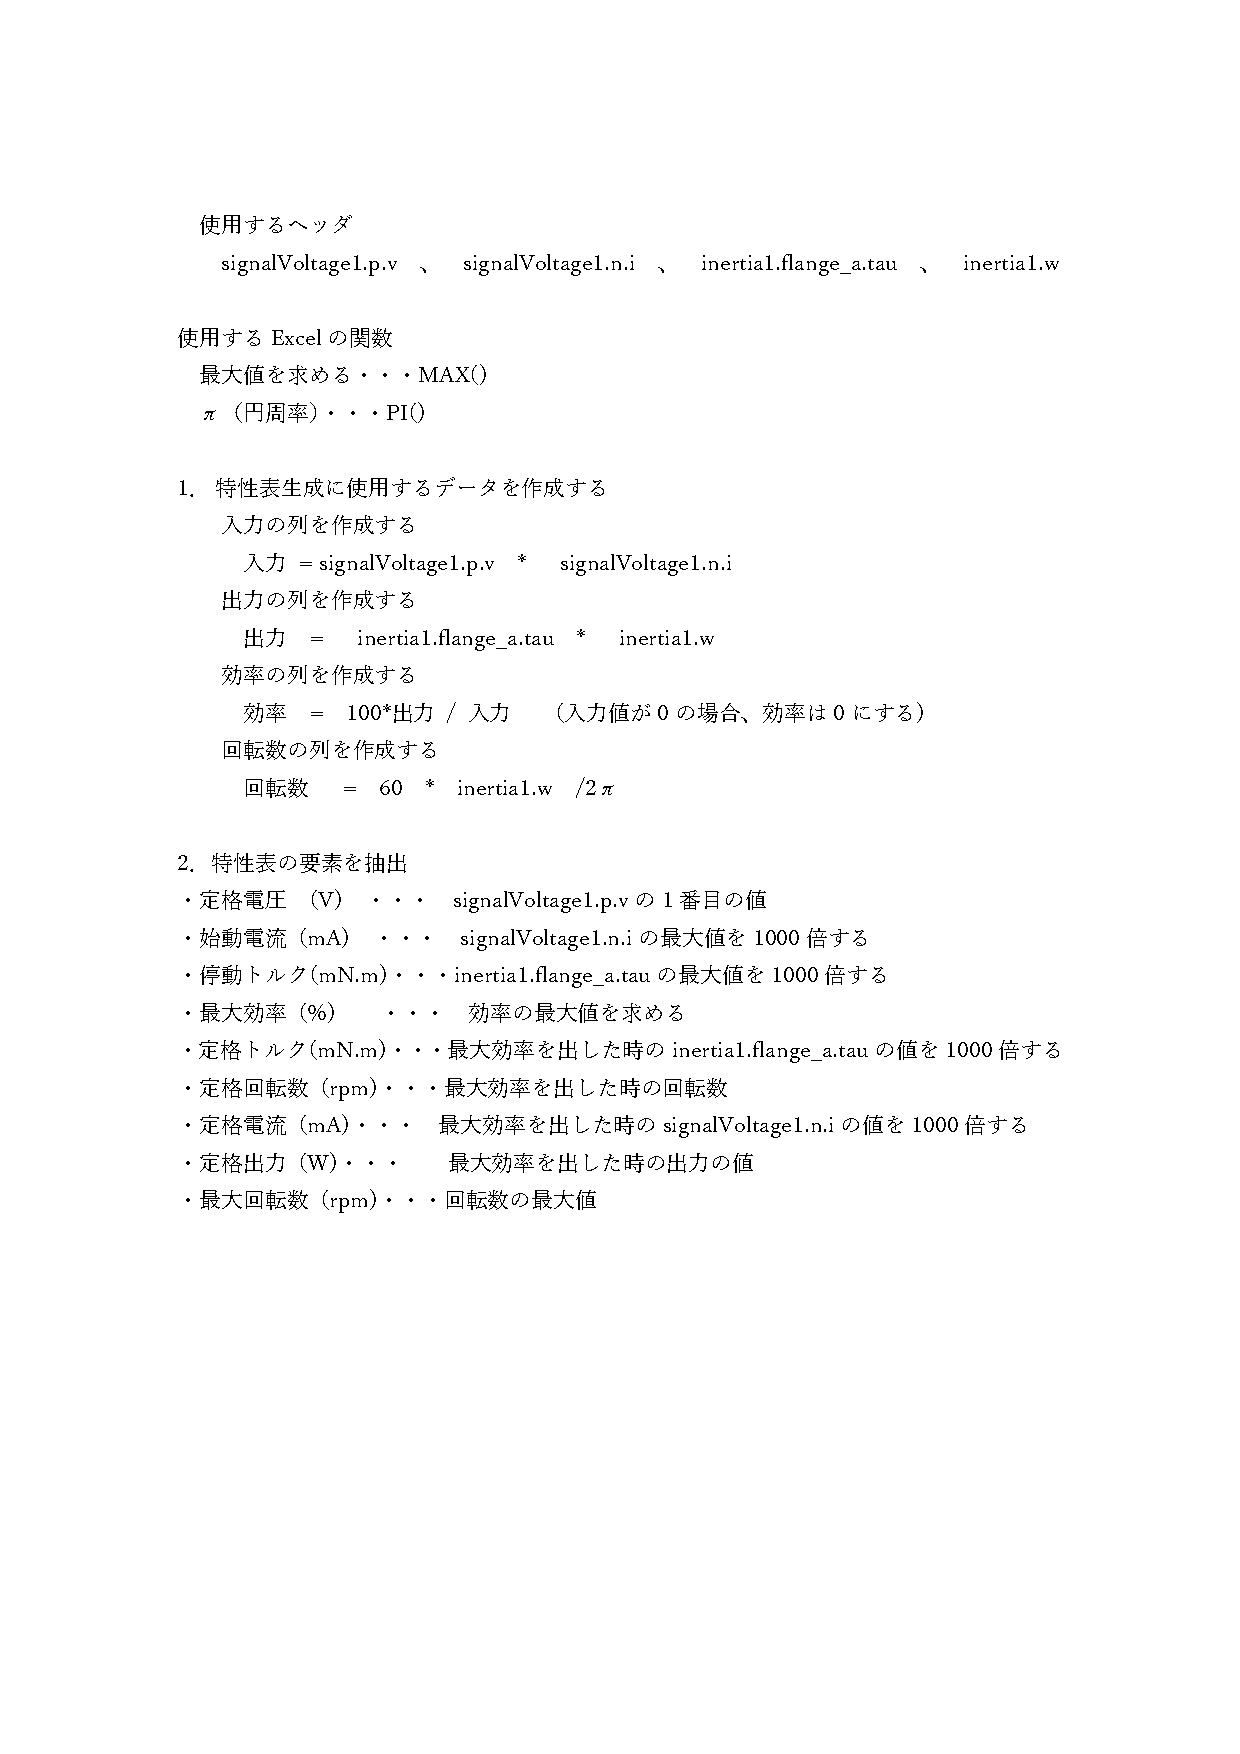
\includegraphics[width=16cm,pagebox=cropbox]{Image/実験方法の説明.pdf}
	}
	\caption{ケースXとケースY で出題する問題}
	\label{fig:mondai}
\end{figure}

\begin{table}[tp]
  \begin{center}
    \caption{ケースXの実験結果}
    \label{resultX}
    \begin{tabular}{c|c|c|c|c|}
    \cline{2-5}
                              & \multicolumn{2}{c|}{ツール未使用} & \multicolumn{2}{c|}{ツール使用} \\ \hline
    \multicolumn{1}{|c||}{被験者} & 回答時間           & 正答率          & 回答時間           & 正答率         \\ \hline\hline
    \multicolumn{1}{|c||}{1}   & 13分5秒           & 56\%         & 57秒           & 100\%         \\ \hline
    \multicolumn{1}{|c||}{2}   & 14分50秒          & 67\%          & 1分20秒          & 100\%         \\ \hline\hline
    \multicolumn{1}{|c||}{平均}   & 13分57.5秒          & 61.5\%          & 1分8.5秒          & 100\%         \\ \hline
    \end{tabular}
  \end{center}
\end{table}

\begin{table}[tp]
  \begin{center}
    \caption{ケースYの実験結果}
    \label{resultY}
    \begin{tabular}{c|c|c|c|c|}
    \cline{2-5}
                              & \multicolumn{2}{c|}{ツール未使用} & \multicolumn{2}{c|}{ツール使用} \\ \hline
    \multicolumn{1}{|c||}{被験者} & 回答時間           & 正答率          & 回答時間           & 正答率         \\ \hline\hline
    \multicolumn{1}{|c||}{3}   & 21分35秒           & 67\%         & 1分10秒           & 100\%         \\ \hline
    \multicolumn{1}{|c||}{4}   & 18分6秒          & 100\%          & 1分58秒          & 89\%         \\ \hline\hline
    \multicolumn{1}{|c||}{平均}   & 19分50.5秒          & 83.5\%          & 1分34秒          & 94.5\%         \\ \hline
    \end{tabular}
  \end{center}
\end{table}

「ケースX」の実験結果から、モータ特性表自動生成ツールを用いない場合の解答時間の平均は「13分57.5秒」である。また、正答率の平均は「61.5\%」である。
一方、モータ特性表自動生成ツールを用いた場合の解答時間の平均は「1分8.5秒」である。また、正答率の平均は「100\%」である。

この結果から、「ケースX」の実験においてモータ特性表自動生成ツールを用いた場合、解答時間の平均は用いなかった場合に比べて「91.8」\%削減できた。
また、モータ特性表自動生成ツールを用いた場合の方が、用いなかった場合に比べて正答率が高いことが示せた。

「ケースY」の実験結果から、モータ特性表自動生成ツールを用いない場合の解答時間の平均は「19分50.5秒」である。また、正答率の平均は「83.5\%」である。
一方、モータ特性表自動生成ツールを用いた場合の解答時間の平均は「1分34秒」である。また、正答率の平均は「94.5\%」である。

この結果から、「ケースY」の実験においてモータ特性表自動生成ツールを用いた場合、解答時間の平均は用いなかった場合に比べて「92.1」\%削減できた。
また、モータ特性表自動生成ツールを用いた場合の方が、用いなかった場合に比べて正答率が高いことが示せた。


これらの結果により、モータ特性表自動生成ツールを用いることで、特定の値を確認するためにかかる時間を削減できることを確認した。
また、モータ特性表自動生成ツールを用いることで、正答率が上がったことを確認できた。正答率が上がった理由として、モータ特性表自動生成ツールを用いることにより、人手によるミスを削減できたことが考えられる。
具体的には、モータ特性表自動生成ツールを用いない場合、手動で表計算ソフトから特定の値を抽出し、計算を行う必要があるため、この過程においてミスが発生する可能性が高まったことが考えられる。
一方、モータ特性表自動生成ツールを用いた場合、ツールが自動で特性表を生成し、提示することにより、人手によるミスが発生する可能性を削減できたことが考えられる。

以上の結果により、モータ特性表自動生成ツールの有用性があることを示せた。また、モータ特性表自動生成ツールを用いることで、特定の値を確認する際に生じるミスを削減できることが確認できた。


\subsection{結果}
本論文で試作したモータ特性表自動生成ツールは、

\section{関連研究}
モデルベースシステム開発で使用されるツールとして、MATLABがある。MATLABはMathWorks社が開発する科学技術計算用のプログラミング言語である。
MATLABは、制御システム、信号処理、ディープラーニングなど幅広い分野の科学技術計算ができる。
また、ブロック線図シミュレータであるSimulinkと連携させることで、モータのモデル化、シミュレーション、グラフの描画ができる。
ただし、モータの性能を決定づける値の算出や、グラフの描画はできるが、モータの特性表の自動生成はできない。
一方、本研究で試作したモータ特性表自動生成ツールは、OpenModelicaのシミュレーション結果から、モータ特性表を自動生成できる。
このため、特性表と特性グラフをまとめたモータ特性表を自動生成できることが試作したツールの利点といえる。

\section{ツールの問題点}

以下に、今回作成したモータ特性表自動生成ツールの問題点を示す。

\begin{itemize}
	\item 対応するモータのモデルが1種類しかない\\
      本論文で試作したモータ特性表自動生成ツールが対象とするのはブラシ付きDCモータである。しかし、ブラシレスモータやACモータなどには対応していない。
      そのため、それらを用いた回路のシミュレーション結果からモータ特性表は作成できない。
		  そのため、対応できる数を増やす必要がある。
    
  \item グラフ
\end{itemize}







